\chapter{Kepo}
Kepo atau \textit{Key Production} adalah sebuah program yang digunakan pada proyek 2 dan proyek 3, berfungsi untuk memudahkan mahasiswa untuk malakukan bimbingan disetiap pertemuan. Kepo menggunakan bahasa pemrograman Python, dan terhubung dengan github melalui repositori dari masing-masing \textit{user}.


\section{Cara Menggunakan Kepo}
\par Cara menggunakan program kepo yaitu:

\begin{enumerate}
\item Langkah pertama buka url if.poltekpos.ac.id jika sudah kemudian klik \textit{read more}.

 \begin{figure}[!htbp]
    \centering
    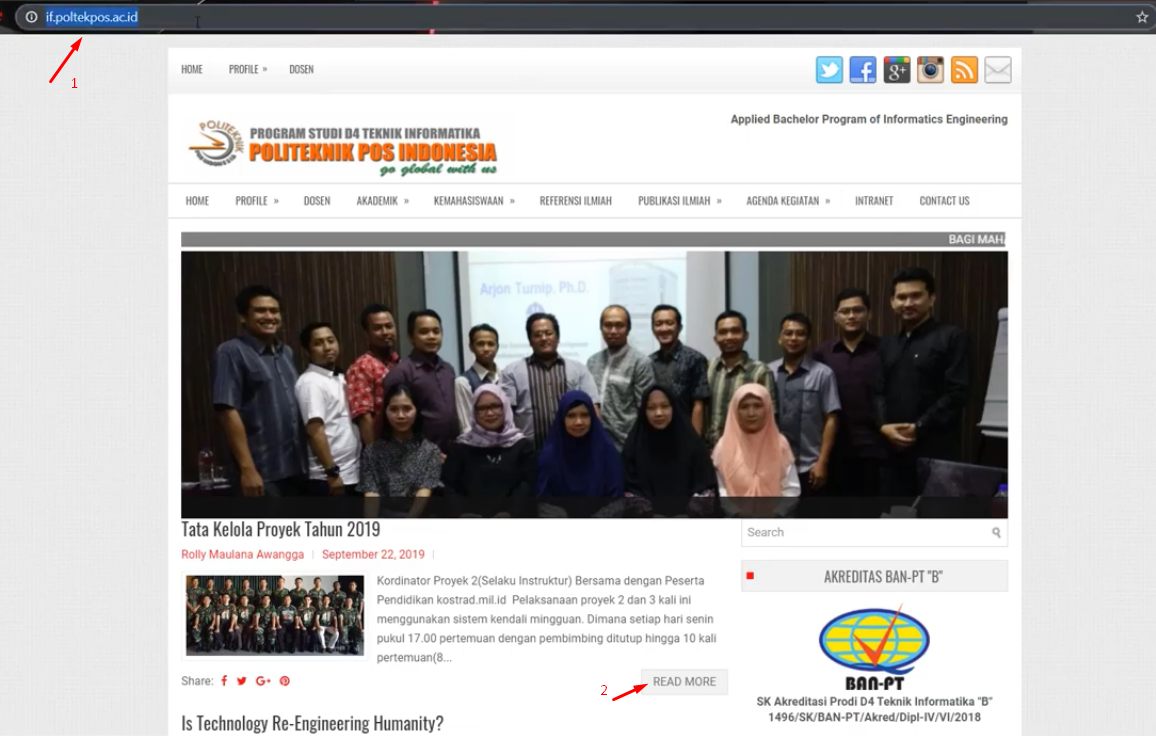
\includegraphics[width=10cm]{figures/if}
    \caption{\textit{Tampilan if.poltekpos.ac.id}}
    
\end{figure} 

\newpage

\item kemudian klik kepo
\begin{figure}[!htbp]
    \centering
    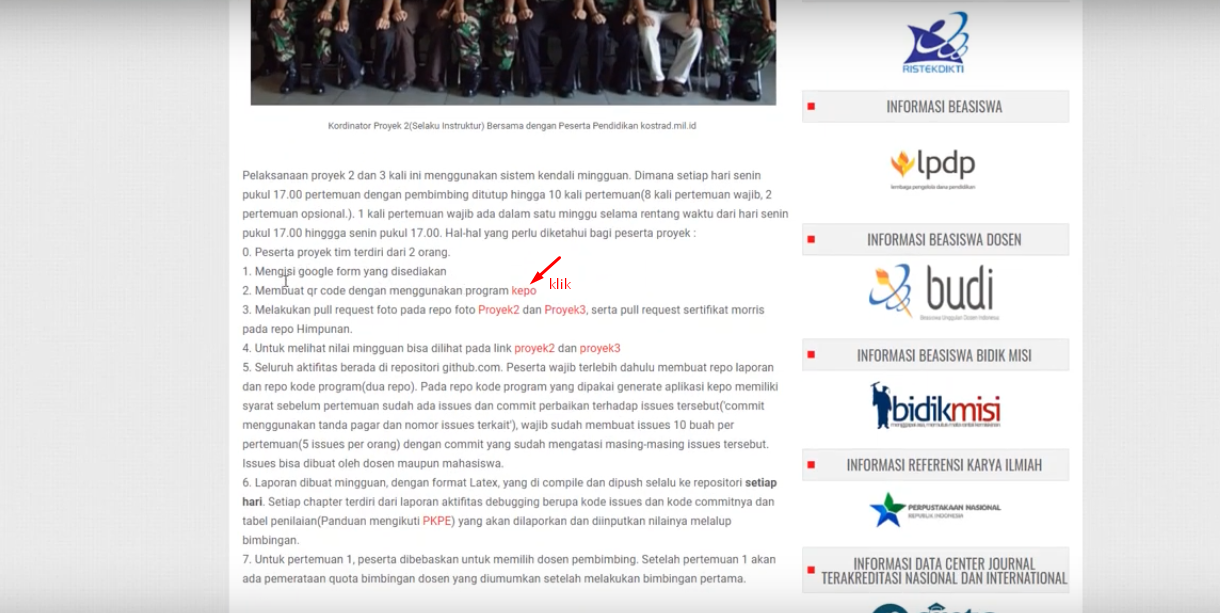
\includegraphics[width=10cm]{figures/klikkepo}
    \caption{\textit{klik kepo}}
    
\end{figure} 

atau bisa juga dengan membuka url https://github.com/awangga/kepo

\begin{figure}[!htbp]
    \centering
    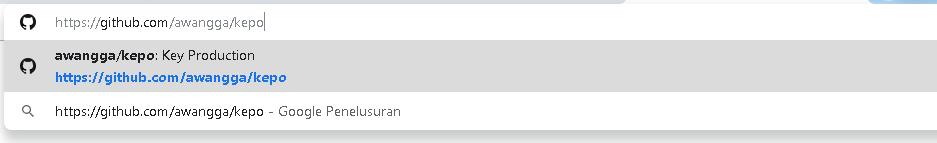
\includegraphics[width=10cm]{figures/kepo}
    \caption{\textit{membuka kepo melalui url}}
\end{figure} 


\item kemudian klik \textit{fork}, jika sudah \textit{clone or download}, atau \textit{download zip}.

\begin{figure}[!htbp]
    \centering
    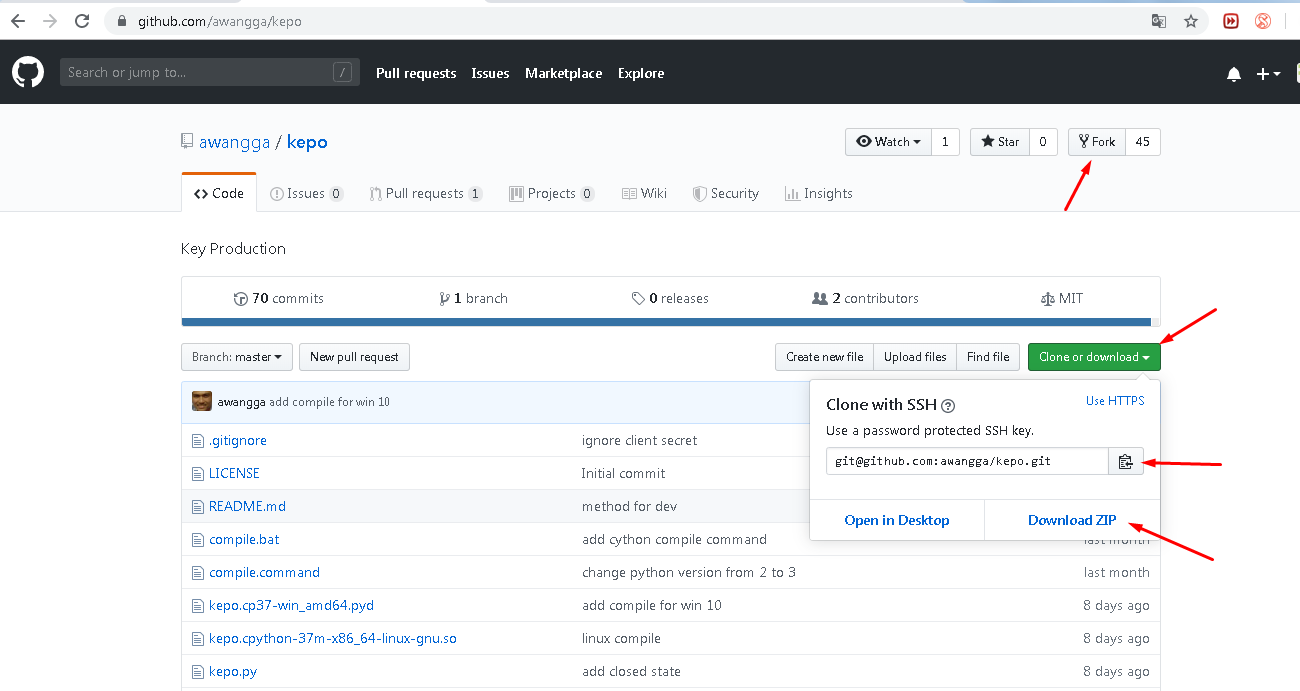
\includegraphics[width=13cm]{figures/tutor}
    \caption{\textit{mendownload kepo}}
\end{figure} 

\newpage

\item buka folder kepo, kemudian \textit{rename} kepo.cp37-winamd64  menjadi kepo.py 
\begin{figure}[!htbp]
    \centering
    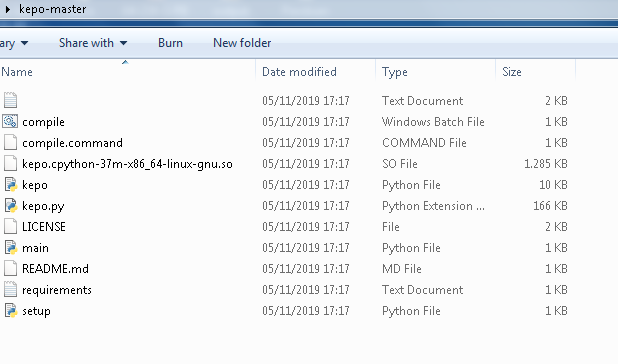
\includegraphics[width=10cm]{figures/rename}
    \caption{\textit{rename}}
\end{figure} 

\item kemudian buka github, lalu buat repo baru. Jika program menggunakan bahasa pemrograman python, pilih python, pada \textit{add a license} pilih MIT license, jika sudah klik \textit{create new repository}.

\begin{figure}[!htbp]
    \centering
    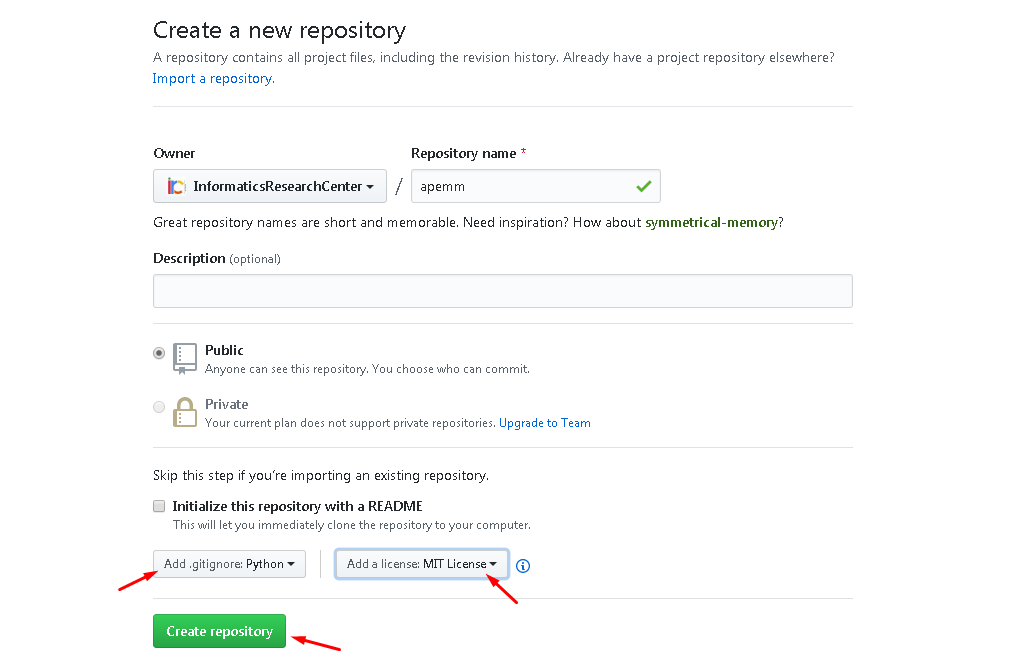
\includegraphics[width=13cm]{figures/newrepo}
    \caption{\textit{create new repository}}
\end{figure} 

\newpage

\item buat 10 \textit{issues} terlebih dahulu.

\begin{figure}[!htbp]
    \centering
    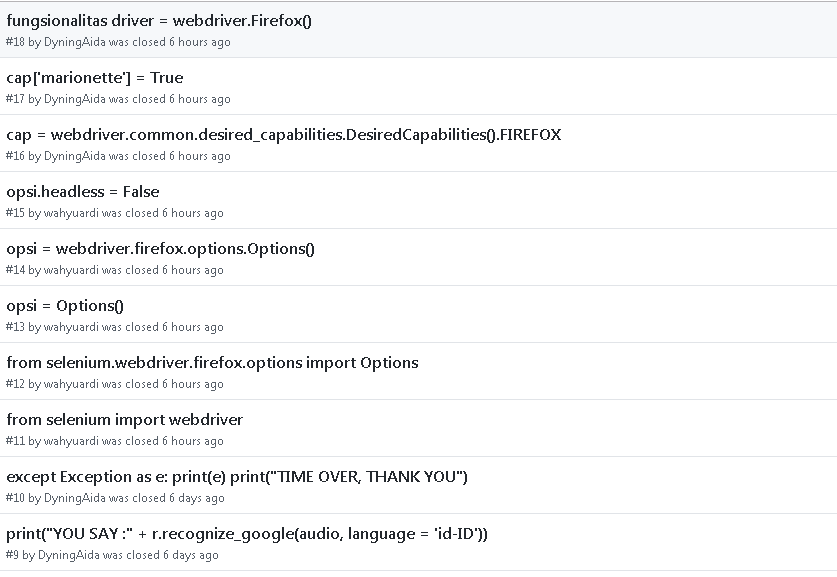
\includegraphics[width=10cm]{figures/issues}
    \caption{\textit{membuat 10 issues}}
\end{figure} 

\item setelah itu \textit{download chrome driver}sesuai versi chrome yang digunakan.

\begin{figure}[!htbp]
    \centering
    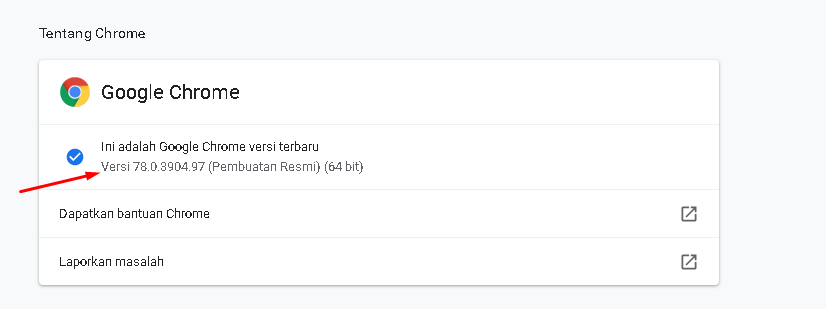
\includegraphics[width=10cm]{figures/versichrome}
    \caption{\textit{versi chrome}}
\end{figure} 

\begin{figure}[!htbp]
    \centering
    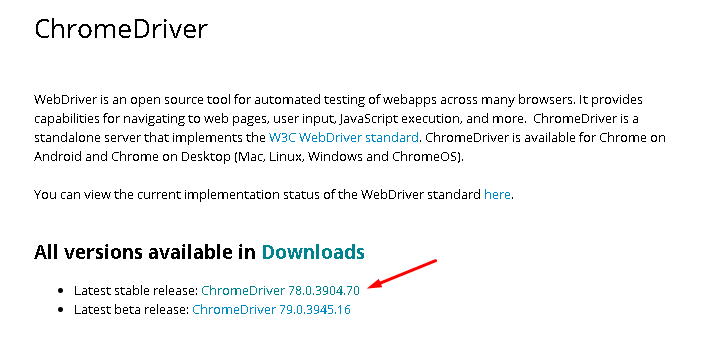
\includegraphics[width=10cm]{figures/chromedriver}
    \caption{\textit{chrome driver}}
\end{figure} 

\newpage

\item letakkan \textit{chrome driver} ke windows-system32

\begin{figure}[!htbp]
    \centering
    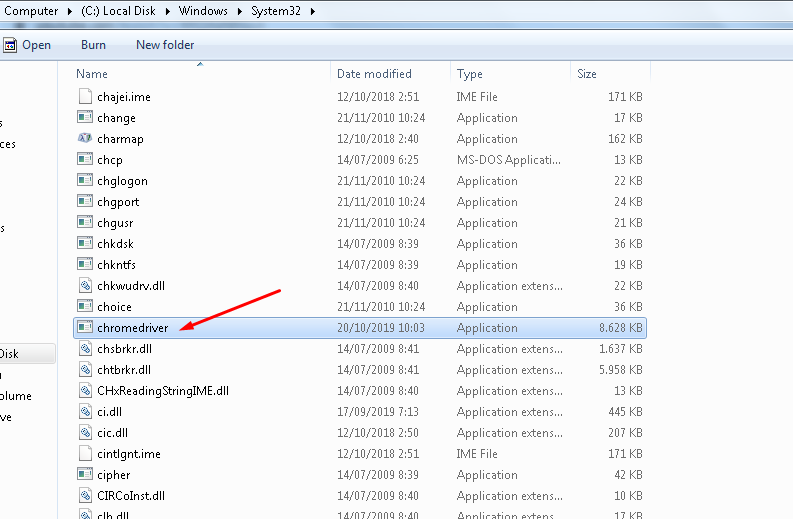
\includegraphics[width=10cm]{figures/pindahchrome}
    \caption{\textit{pindahkan chrome driver ke windows system32}}
\end{figure} 

\item kemudian buka folder kepo, lalu pada ketik CMD untuk mempermudah.

\begin{figure}[!htbp]
    \centering
    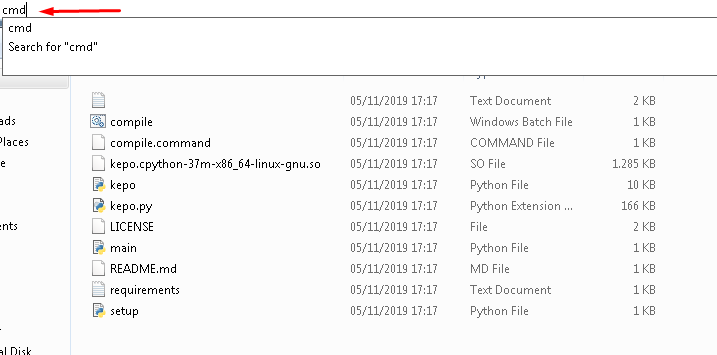
\includegraphics[width=10cm]{figures/folderkepo}
    \caption{\textit{membuka folder kepo}}
\end{figure} 

\newpage

\item pada cmd ketikkan perintah pip install -r requirements.txt dan
python main.py

\begin{figure}[!htbp]
    \centering
    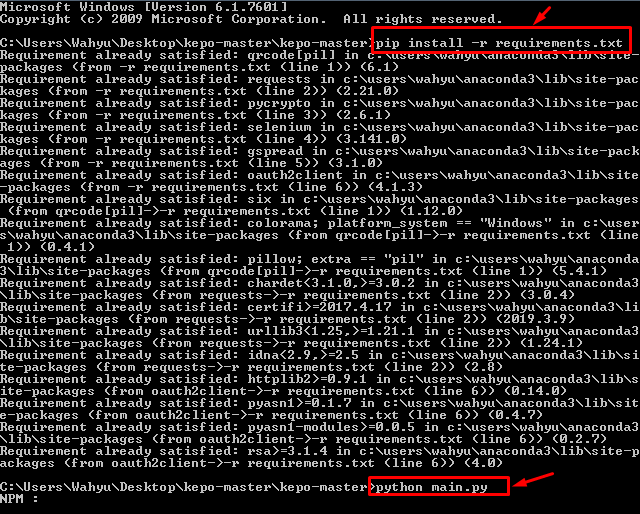
\includegraphics[width=10cm]{figures/cmd}
    \caption{\textit{cmd}}
\end{figure}

\item kemudian \textit{input} 

\begin{figure}[!htbp]
    \centering
    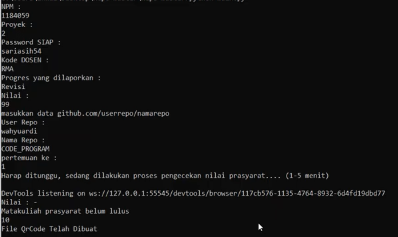
\includegraphics[width=10cm]{figures/inputt}
    \caption{\textit{input}}
\end{figure}

\newpage

\item qrcode akan muncul di folder kepo

\begin{figure}[!htbp]
    \centering
    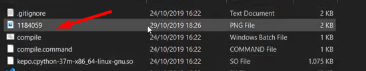
\includegraphics[width=10cm]{figures/qrcode}
    \caption{\textit{file qrcode}}
\end{figure}

kemudian klik file qrcodenya, dan ini adalah qrcode tersebut.
\begin{figure}[!htbp]
    \centering
    
\includegraphics[width=10cm]{figures/iniqrcode}
    \caption{\textit{qrcode}}
\end{figure}

\end{enumerate}

\newpage

\subsection{Jika issues kurang dari 10}
\par jika \textit{issues} kurang dari 10 maka :

\begin{figure}[!htbp]
    \centering
    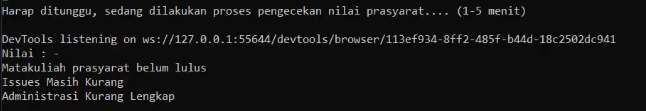
\includegraphics[width=15cm]{figures/issueskurang}
    \caption{\textit{issues kurang dari 10}}
\end{figure}

